%%==========================================================================
%% This is the very first version of a Streetwise LaTeX template. By
%% chosing the document class, it is easily convertible to a two-column IEEE
%% paper format, provided any conflicting packages and (new)commmands are
%% removed.
%%
%% Erwin de Gelder, January 6, 2018
%%==========================================================================

%%==========================================================================
%% Title:
%% Author(s):
%% To be published in:
%% Date of submission:
%% Date of submission R1:
%% Date of submission R2:
%% Date of final submission:
%%==========================================================================


%% Generic
\documentclass[10pt,final,a4paper,oneside,onecolumn]{article}

%% IEEE
%% Document class options: replace "draftcls" by "final" for final document.
%% All other options may just as well be omitted because they are the default values.
%\documentclass[10pt,final,journal,letterpaper,twoside,twocolumn]{IEEEtran}


%%==========================================================================
%% Document automation
%%==========================================================================

\def\reptitle{Go/No Go report}
\def\repauthor{Erwin de Gelder}


%%==========================================================================
%% Packages
%%==========================================================================

\usepackage[a4paper,left=3.5cm,right=3.5cm,top=3cm,bottom=3cm]{geometry} %% change page layout; remove for IEEE paper format
\usepackage[T1]{fontenc}                        %% output font encoding for international characters (e.g., accented)
\usepackage[cmex10]{amsmath}                    %% math typesetting; consider using the [cmex10] option
\usepackage{amssymb}                            %% special (symbol) fonts for math typesetting
\usepackage{amsthm}                             %% theorem styles
\usepackage{dsfont}                             %% double stroke roman fonts: the real numbers R: $\mathds{R}$
\usepackage{mathrsfs}                           %% formal script fonts: the Laplace transform L: $\mathscr{L}$
\usepackage[pdftex]{graphicx}                   %% graphics control; use dvips for TeXify; use pdftex for PDFTeXify
\usepackage{array}                              %% array functionality (array, tabular)
\usepackage{upgreek}                            %% upright Greek letters; add the prefix 'up', e.g. \upphi

\usepackage[utf8]{inputenc}   				 	%% utf8 support (required for biblatex)
\usepackage[style=ieee,doi=false,isbn=false,url=false,date=year,minbibnames=15,maxbibnames=15,backend=biber]{biblatex}
%\renewcommand*{\bibfont}{\footnotesize}		%% Use this for papers
\setlength{\biblabelsep}{\labelsep}
\bibliography{../bib}

\usepackage{stfloats}                           %% improved handling of floats
\usepackage{multirow}                           %% cells spanning multiple rows in tables
%\usepackage{subfigure}                         %% subfigures and corresponding captions (for use with IEEEconf.cls)
%\usepackage{subfig}                             %% subfigures (IEEEtran.cls: set caption=false)
\usepackage{fancyhdr}                           %% page headers and footers
\usepackage[official,left]{eurosym}             %% the euro symbol; command: \euro
\usepackage{appendix}                           %% appendix layout
\usepackage{xspace}                             %% add space after macro depending on context
\usepackage{verbatim}                           %% provides the comment environment
\usepackage[dutch,USenglish]{babel}             %% language support
\usepackage{wrapfig}                            %% wrapping text around figures
\usepackage{longtable}                          %% tables spanning multiple pages
\usepackage{pgfplots}                           %% support for TikZ figures (Matlab)
\usepackage[breaklinks=true,hidelinks,          %% implement hyperlinks (dvips yields minor problems with breaklinks;
            bookmarksnumbered=true]{hyperref}   %% IEEEtran: set bookmarks=false)
%\usepackage[hyphenbreaks]{breakurl}            %% allow line breaks in URLs (don't use with PDFTeX)
\usepackage{lmodern} 
\usepackage{etoolbox}							%% Needed for apptocmd later
\usepackage[capitalize]{cleveref}
\usepackage{units}
\usepackage{subcaption}
\usepackage{csquotes}							%% Quoted texts are typeset according to rules of main language
\usepackage{xparse}

%%==========================================================================
%% Fancy headers and footers
%%==========================================================================

\newtoggle{standalone}
\toggletrue{standalone}
\pagestyle{fancy}                                       %% set page style
\fancyhf{}                                              %% clear all header & footer fields
\iftoggle{standalone}{%
	\fancyhead[L]{Go/No Go} %% define headers (LE: left field/even pages, etc.)
	\fancyhead[R]{Erwin de Gelder, October 2, 2018}                   %% similar
	\fancyfoot[C]{\thepage}                                 %% define footer
	\setlength{\headheight}{18pt}
	\renewcommand*{\headrulewidth}{0.25pt}                  %% header line width
	%% Redefine the default "plain" page style (automatically activated by \maketitle, \section, ...)
	\fancypagestyle{plain}{%
		\fancyhf{}
		\renewcommand{\headrulewidth}{0pt}
		\renewcommand{\footrulewidth}{0pt}
		\setlength{\headheight}{36pt}
	}
}{%
	\renewcommand*{\headrulewidth}{0pt}                  	%% No line in this case
	%% Redefine the default "plain" page style (automatically activated by \maketitle, \section, ...)
	\fancypagestyle{plain}{%
		\fancyhf{}
	}
}
\renewcommand*{\footrulewidth}{0pt}                     %% footer line width


%%==========================================================================
%% TikZ figures
%%==========================================================================

\newlength\figurewidth
\setlength\figurewidth{0.35\textwidth}              %% set figure width
\newlength\figureheight
\setlength\figureheight{0.3\textwidth}              %% set figure height
\pgfplotsset{every axis/.append style={
    scaled y ticks=false,
    scaled x ticks=false,
    y tick label style={/pgf/number format/fixed},
    x tick label style={/pgf/number format/fixed},
    legend style={font=\small}},
    compat=1.9}                                     %% PGFPlots package options
\usetikzlibrary{shapes.geometric, arrows, arrows.meta}
\usepgfplotslibrary{groupplots}
%\usetikzlibrary{external}                           %% Create pdf figures from TikZ. Use PDFTeXify ...
%\tikzexternalize[prefix=./tikz/]                    %% ... with --tex-option=--shell-escape switch.
%\tikzset{external/force remake}                    %% force pdf figure update


%%==========================================================================
%% User-defined commands
%%==========================================================================

\newcommand*{\mat}[1]{\mathbf{#1}}                              %% matrix/vector notation
\newcommand*{\matsym}[1]{\boldsymbol{#1}}                       %% matrix/vector notation for Greek letters
\newcommand*{\T}{^{\scriptscriptstyle\mathsf{T}}}               %% transpose operator
\newcommand*{\Hr}{^{\scriptscriptstyle\mathsf{H}}}              %% conjugate transpose operator
\newcommand*{\ud}{\mathrm{\,d}}                                 %% differential operator (upright d)
\newcommand*{\defeq}{\mathrel{\mathop:}=}                       %% definition sign :=
\newcommand*{\eqdef}{=\mathrel{\mathop:}}                       %% definition sign =:
\newcommand*{\ip}[2]{\left\langle#1\,{,}\,#2\right\rangle}      %% inner product
\newcommand*{\real}[1]{\mathrm{Re}(#1)}                         %% real part
\newcommand*{\imag}[1]{\mathrm{Im}(#1)}                         %% imaginary part
\newcommand*{\lsup}[1]{{}^{#1}\!}                               %% left superscript
\newcommand*{\hi}[1]{$^\text{#1}$}                              %% superscript in normal text
\newcommand*{\lo}[1]{$_\text{#1}$}                              %% subscript in normal text
\newcommand*{\w}[1]{\mathrm{#1}}                                %% multiple character super-/subscript in math mode
\newcommand*{\capskip}{\vspace{-12pt}}                          %% caption skip for figures with subfloats
\newcommand*{\etal}{et al.}                                     %% may be required for Natbib bibliography styles
\renewcommand*{\qedsymbol}{$\blacksquare$}                      %% redefine the end-of-proof symbol
\renewcommand*{\labelitemi}{$\bullet$}                          %% first level item list bullet
\renewcommand*{\labelitemii}{$-$}                               %% second level item list bullet
%\renewcommand*{\theenumi}{\textit{\roman{enumi}}}               %% first level enumerator
\renewcommand*{\labelenumi}{\theenumi.}
\renewcommand*{\theenumii}{\textit{\alph{enumii}}}              %% second level enumerator
\renewcommand*{\labelenumii}{\theenumii.}
\DeclareMathOperator{\tr}{tr}                                   %% trace of a matrix
\DeclareMathOperator{\sgn}{sgn}                                 %% signum function
\DeclareMathOperator{\atan}{atan}                               %% arc tangent

\newcommand{\class}[1]{\emph{#1}}

\crefname{figure}{Figure}{Figures}
\crefname{equation}{}{}
\Crefname{equation}{Equation}{Equations}

%%==========================================================================
%% User-defined environments
%%==========================================================================

\theoremstyle{plain}\newtheorem{definition}{Definition}[section]    %% definition
                    \newtheorem{theorem}{Theorem}[section]          %% theorem
                    \newtheorem{lemma}[theorem]{Lemma}              %% lemma
                    \newtheorem{corollary}[theorem]{Corollary}      %% corollary
                    \newtheorem{assumption}{Assumption}[section]    %% assumption
                    \newtheorem{condition}{Condition}[section]      %% condition
\theoremstyle{definition}\newtheorem{example}{Example}[section]     %% examples
\theoremstyle{remark}\newtheorem{remarkenv}{Remark}[section]        %% remarks
\newenvironment{remark}{\begin{remarkenv}}%
                       {\hfill$\blacklozenge$\end{remarkenv}}       %% end remark with a lozenge
\newenvironment{reviewer}{\itshape}{\upshape}                       %% environment for reviewer's comments


%%==========================================================================
%% Miscellaneous
%%==========================================================================

\graphicspath{{./../}{./figures/}{./more_figures/}} %% (graphicx) directory path for figures
%\setlength{\parindent}{0pt}                        %% no paragraph indentation
%\setlength{\parskip}{2ex}                          %% create empty line between paragraphs
%\interdisplaylinepenalty=2500                      %% (amsmath) allow for page breaks within multiline equations
%\numberwithin{equation}{section}                   %% (amsmath) include section number in equation numbering
%\numberwithin{figure}{section}                     %% (amsmath) include section number in figure numbering
%\numberwithin{table}{section}                      %% (amsmath) include section number in table numbering
\addtolength{\arraycolsep}{-0.5mm}                  %% squeeze matrix columns a little
\fnbelowfloat                                       %% (stfloats) put footnote below a float at the page bottom
\urlstyle{same}                                     %% (hyperref) use current font for URLs
\hypersetup{pdftitle={\reptitle},
            pdfauthor={\repauthor}}                 %% (hyperref) pdf properties title and author
%\raggedbottom                                      %% don't add inter-paragraph spacing to achieve \textheight
%\setlength\subfigcapskip{-3pt}                     %% (subfigure) distance between subfloat and subcaption
%\setlength\subfigbottomskip{-3pt}                  %% (subfigure) distance between subcaption and caption
%\renewcommand*{\subcapsize}{\small}                %% (subfigure) subcaption font size
\renewcommand*{\thesubfigure}{(\alph{subfigure})}   %% (subfig) implement 1(a) instead of 1a ...as subfigure reference
\captionsetup[subfloat]{labelformat=simple}        %% ... as subfigure reference
%\captionsetup[subfloat]{
%    farskip=0pt,
%    nearskip=8pt,
%    captionskip=1.5pt,
%    labelfont={small,bf},
%    textfont=small}                                %% (subfig) subfloat caption format
%\captionsetup[figure]{
%    labelfont={small,bf},
%    textfont=small}                                %% (subfig/caption) figure caption format
%\captionsetup[table]{
%    aboveskip=2pt,
%    labelfont={small,bf},
%    textfont={small,sc}}                           %% (subfig/caption) table caption format
\apptocmd{\thebibliography}{\raggedright}{}{}		%% Suppress badness warnings in bibliography


% Table stuff
\usepackage{booktabs}
\usepackage{tabularx}
\setlength{\heavyrulewidth}{0.1em}
\newcommand{\otoprule}{\midrule[\heavyrulewidth]}

%\usepackage{changebar}  %% When including the package earlier, it does not work for some reason...

%%==========================================================================
%% Begin document
%%==========================================================================

\begin{document}

\selectlanguage{USenglish}

\title{\textbf{\reptitle}}
\author{\repauthor}
\date{October 2, 2018}
\maketitle

\tableofcontents

\newpage

\section{Biography}
\label{sec:bio}

My academic career started when I began my bachelor in Mechanical Engineering at the Delft University of Technology (DUT) in 2008. I received my B.Sc.\ in 2011 (cum laude). After my bachelor, I immediately started with a master in Systems and Control at DUT. A break of one year allowed me as a member of the board of the Formula Student team of DUT to work on the most awesome race car. In 2014, I receive my M.Sc.\ degree (cum laude) after graduating under the supervision of Michel Verhaegen \cite{deGelder2015sabre}.

After graduating from the DUT, I wanted to continue my academic career and, therefore, I started working at the Netherlands Organisation for Applied Scientific Research (TNO). This gave me the opportunity to continue with research while working on various projects, among which applying machine learning for the classification of car-cyclist scenarios \cite{cara2015carcyclist}, working on cooperative driving (e.g., with the Grand Cooperative Driving Challenge), researching personalized Advanced Driving Assistance Systems using the study of naturalistic driving data \cite{gelder2016pacc}, and the assessment of Automated Driving (AD) functions using real-world data \cite{deGelder2017assessment}.

When I was working on various projects related to the assessment of AD functions, my enthusiasm indicated that this was the topic I wanted to focus on for a longer period. For me, having this focus was a prerequisite for allowing me to pursue a PhD degree. As a result, I started as a PhD candidate in October 2017. I chose Bart De Schutter as my supervisor from the DUT as he also supervised Olaf Gietelink with his PhD on a similar topic \cite{gietelink2007phd}. Given their experience in the field of research, Jan-Pieter Paardekooper and Olaf Op den Camp are the logical choices as supervisors from TNO.

Having started my pursue to a PhD degree, TNO started a collaboration with the Centre of Excellence of Testing and Research at the Nanyang Technological University (CETRAN) to work on a certification procedure for automated vehicles (AVs). As a result, I am now stationed in Singapore to work on a scenario-based safety assessment framework for auto AVs \cite{ploeg2018cetran}.

\section{Research}
\label{sec:research}


\subsection{Introduction}
\label{sec:introduction}

% Automated Vehicles are introduced (in Singapore)
The development of automated vehicles (AVs) has made significant progress. It is expected that before 2020, automated and autonomous vehicles will be introduced in controlled environments, whereas autonomous vehicles will be mainstream by 2040 \cite{madni2018autonomous} or earlier \cite{bimbraw2015autonomous}. Especially in densely populated cities such as Singapore, there is a need for automated vehicles to increase traffic safety and traffic efficiency by enabling flexible, automated, mobility-on-demand systems \cite{spieser2014toward}, scheduled services for public transport needs, and automated freight and service vehicles to support 24 hours operations and labor shortage needs.

% Assessment of AVs is important
An important aspect in the development of AVs is the safety assessment of the AVs \cite{bengler2014threedecades, stellet2015taxonomy, putz2017pegasus, wachenfeld2016release}. For legal and public acceptance of AVs, a clear definition of system performance is important, as are quantitative measures for the system quality. The more traditional methods \cite{ISO26262, response2006code}, used for evaluation of driver assistance systems, are no longer sufficient for assessment of the safety of higher level AVs, as it is not feasible to complete the quantity of testing required by these methodologies \cite{wachenfeld2016release}. Therefore, the development of assessment methods is important to not delay the deployment of AVs \cite{bengler2014threedecades}.

% Scenario-based approach
One proposed way to assess safety is to test drive AVs in real traffic, observe their performance, and make statistical comparisons to human driver performance. However, this requires AVs to drive hundreds of millions of kilometers and sometimes hundreds of billions of kilometers to demonstrate their reliability in terms of fatalities and injuries \cite{kalra2016driving}. It does not seem to be feasible to drive these millions of kilometers with the increased speed of development of automated driving (AD) functions and the high level of safety requirements that are expected from these functions. As an alternative, a scenario-based assessment is adopted \cite{putz2017pegasus, stellet2015taxonomy, deGelder2017assessment, ploeg2018cetran, elrofai2018scenario}. 
% Scenarios are obtained with data
These test-scenarios can be knowledge-driven or data-driven \cite{stellet2015taxonomy}. A drawback of knowledge-based test-scenarios is that it does not allow to generalize the results to the performance of the system-under-test when operating in traffic, i.e. the test cases may not be valid or representative for real-world traffic. A data-driven approach does allow to
generalize the results, but here the challenge is to extract the interesting, e.g., performance critical, scenarios from the data, such that the number of simulations is still limited \cite{deGelder2017assessment}.

\subsection{Focus of research}
\label{sec:focus}

% Use summary Go/No Go meeting


\subsection{Preliminary results}
\label{sec:results}




\subsection{Submitted paper}
\label{sec:paper}


\subsection{Outlook}
\label{sec:outlook}

\section{Personal comments}
\label{sec:personal}

My PhD project is now almost one year underway, so this is a good time to reflect how I personally experienced this. When looking back, I realize that there are some areas I can improve upon. Few points for improvements are mentioned in \cref{sec:evaluation}, but first some other personal comments are listed:
\begin{itemize}
	\item I am very satisfied with my choice for Bart De Schutter as a supervisor from the TUD and I am grateful that he accepted to supervise me. I am amazed by the comprehensiveness and accurateness of his comments and his patience to explain his remarks (again and again).
	\item I am also very satisfied with my supervisors from TNO, Jan-Pieter Paardekooper and Olaf Op den Camp. The discussions I have with them are a huge inspiration for me.
	\item Most importantly, I am still enjoying my pursue for a PhD degree every day. I still feel enthusiasm when talking about my PhD and I am very eager to continue every day with my PhD and work at TNO. 
\end{itemize}

\subsection{Self-evaluation}
\label{sec:evaluation}

I am aware that there are many points for improvement. To limit the following list, I selected two points that probably deserve most attention.

\begin{itemize}
	\item \emph{Time and expectation management}: In theory, I work five days a week: two days for my PhD at the Nanyang Technological University (NTU), two days for CETRAN at the NTU, and one day for projects of TNO at the TNO office. In practice, however, my activities are a bit scattered. For example, it sometimes happens that I can only work on my PhD for one hour a day. It turned out te be hard to do proper research in one hour. Furthermore, due to internal deadlines, I sometimes have no time to work on my PhD at all for one or two weeks.
	
	I noticed that it worked best if I can focus for a longer period on my PhD, e.g., for few days or a week with no other appointments in between. This is perfectly achievable, but it needs better time and expectation management from my side and I might need to change the expectations of other stakeholders (see next item). With a better planning, I think it should be possible to have more time for my PhD and to work for longer periods continuously on my PhD.
	
	Regarding expectation management, too often I say ``yes'' when asked to finish something before the end of the week, resulting in postponing my PhD work with another week. I need to be more assertive and be able to say ``no''. Furthermore, sometimes I underestimate the time I need to finish something, so I need to better estimate the time I need before saying ``yes''.
	
	\item \emph{Stakeholder management}: As with every project, several stakeholders are involved with my PhD project, see \cref{fig:stakeholders}. Regarding my work, I identified four important stakeholders, each with different demands:
	\begin{itemize}
		\item \emph{TNO Singapore}: Obtain good results with CETRAN and acquire new projects.
		\item \emph{TNO Netherlands}: Develop the methodology of generating test cases based on real-world data.
		\item \emph{CETRAN}: Develop a certification procedure for AVs.
		\item \emph{TUD}: Assuring that the work is scientifically correct and relevant.
		\item \emph{Myself}: Find satisfaction with the work done.
	\end{itemize}
	The work for my PhD needs to be useful for all these stakeholders. Sometimes, the work I do is only useful for a limited number of stakeholders, which makes my work less efficient.
	
	Next to the stakeholders regarding my work, there are stakeholders that involve my personal life (see \cref{fig:stakeholders}) and that have a direct influence on my PhD project, being my girlfriend, my family, my friends, and sports (I am member of the board of the table tennis club in Helmond). Although I feel full support from these stakeholders regarding my PhD and my ``Singapore campaign'', it sometimes leads to conflicts as all these stakeholders sometimes demand my precious time.
	
	One way to improve on my stakeholder management is communicating clearly the expectations and objectives of myself and the other stakeholders among the different stakeholders. To further improve on this, I want to follow a course on stakeholder management.
\end{itemize}

\begin{figure}
	\centering
	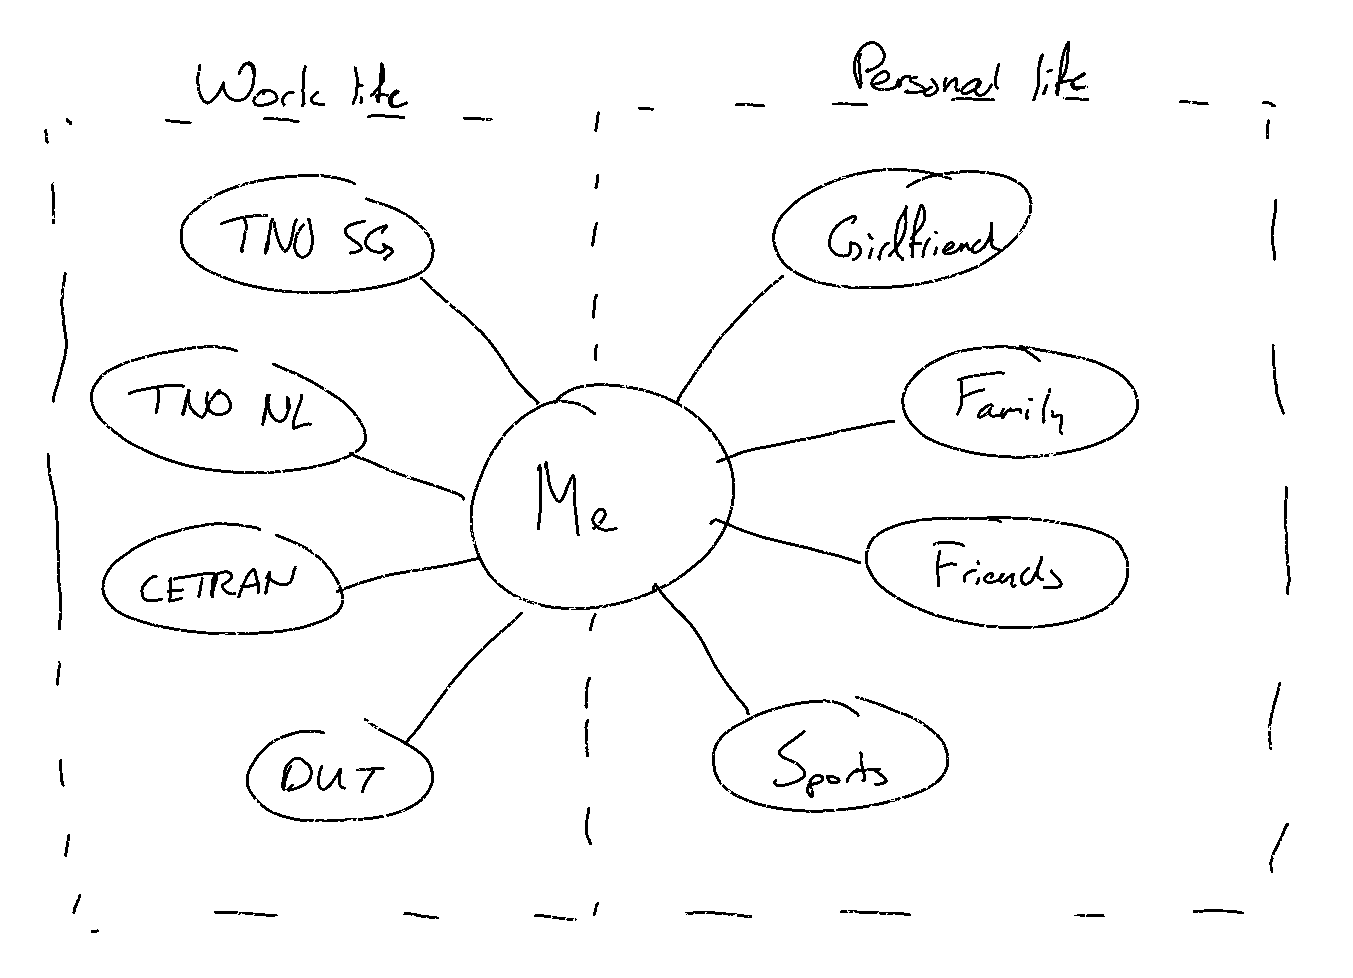
\includegraphics[width=\linewidth]{figures/stakeholders}
	\caption{Overview of the different stakeholders that are involved in my PhD project, either relating to my work or personal life.}
	\label{fig:stakeholders} 
\end{figure}

%\subsection{Graduate school}
%\label{sec:graduate school}



\printbibliography

\end{document} 